\chapter{Referencial Teórico}\label{sec:ref_teorico}

O problema de casamento de padrão consiste em buscar as ocorrências de uma dada cadeia de caracteres $p$ em um texto $t$. Nele há uma janela, na qual o padrão é buscado, que possui o mesmo tamanho do padrão e é movida da esquerda para a direita pelo texto.

Há dois tipos de problemas de casamento de padrão:
\begin{itemize}
    \item Casamento exato de padrão
    \item Casamento aproximado de padrão
\end{itemize}

O problema de casamento exato de padrão é definido como encontrar todas as ocorrências $t_{j',j} = t_{j'}..t_{j}$ de um padrão $p = p_{1},..,p_{m}$ em um texto $t = t_{1},..,t_{n}$, sendo $m \leq n$.

Já o problema de casamento aproximado de padrão é definido como encontrar todas as subcadeias de caracteres $t_{j',j} = t_{j'}..t_{j}$ de um texto $t = t_{1},..,t_{n}$ cuja distância de edição para um padrão $P = p_{1},..,p_{m}$ esteja dentro de um limiar $\tau$, ou seja, $ed(t_{j',j}, P) \leq \tau$, sendo $ed(s_{1}, s_{2})$ uma função que calcula a distância de edição entre $s$ e $t$. Nesse caso, o tamanho de cada ocorrência pode variar de $m - \tau$ até $m + \tau$. A distância de edição entre duas cadeias de caracteres $s_{1}$ e $s_{2}$ é definida como \textit{o menor número de operações para transformar $s_{1}$ em $s_{2}$}. As operações mais permitidas comumente nesse contexto seguem a chamada \textit{distância de edição de Levenshtein} \citep{levenshtein1966binary}, que são:

\begin{enumerate}
    \item \textbf{Inserção} de um único caractere. Se $s = ac$ então inserir o símbolo $b$ na posição do meio, por exemplo, produz $s = abc$. Também pode ser representada por $\epsilon \to b$.
    \item \textbf{Deleção} de um único caractere torna $s = abc$ em $s = bc$, por exemplo. Também pode ser representada por $a \to \epsilon$.
    \item \textbf{Substituição} de um caractere $b$ por um símbolo $q \neq b$ modifica  $s = abc$ para $s = aqc$. Também pode ser representada por $b \to q$.
\end{enumerate}

Esse problema é encontrado em  várias aplicações práticas,  por exemplo em buscas por sequências de DNA, ou para prover sugestões de correções de erros de digitação cometidos pelos usuários ao realizarem consultas em sistemas de busca.

\newpage
\section{Problema da Complementação Automática de Consultas Tolerante a Erros}

O problema de complementação automática de consultas tolerante a erros pode ser visto como uma versão especializada do problema de casamento de padrão. Seja \textit{p} uma cadeia de caracteres que representa uma consulta de prefixo já digitada pelo usuário, um conjunto de cadeias de caracteres \textit{S} que representa a base de consultas e $\tau$ um limite máximo de distância de edição tolerado. O problema consiste em encontrar todos os elementos de \textit{S} que correspondem à \textit{p} com no máximo $\tau$ erros.

Um elemento $s$ qualquer do conjunto $S$ possui vários prefixos. Se $s = ``sapato"$, seus possíveis prefixos são \textit{\{``s'', ``sa'', ``sap'', ``sapa'', ``sapat'', ``sapato''\}}. Se qualquer um deles puder ser transformado em $p$ com um número de operações menor ou igual à $\tau$, então $s$ corresponde à $p$ com no máximo $\tau$ erros, e fará parte da resposta do problema. A solução para o problema deve atender a uma restrição de computar os resultados em um tempo menor que a velocidade média de digitação de um usuário comum, a qual é aproximadamente $100ms$ \citep{ji2009efficient}.

\section{Opções de Solução para o Problema de CATE}

As soluções para o problema de casamento de padrão podem ser divididas em dois grupos. O primeiro engloba abordagens baseadas em busca sequencial por toda a base de consultas. O segundo grupo consiste em abordagens que criam índices a partir da base de consultas em um momento anterior ao processamento de requisições. 

\subsection{Busca Sequencial}
\label{sec:sequential_search}

Os algoritmos de busca sequencial que não utilizam índices consistem em percorrer todos os itens da base de consultas, e comparar o prefixo de consulta com cada item, para determinar quais consultas devem fazer parte da resposta. No contexto de CATE, essa comparação consiste em verificar se o prefixo consultado pode ser transformado em algum dos possíveis prefixos da consulta com no máximo $\tau$ operações. Descreveremos a seguir uma solução de busca sequencial baseada em um algoritmo de programação dinâmica proposto por \cite{levenshtein1966binary}. 

Um método conhecido para calcular a distância de edição entre duas cadeias de caracteres $A$ e $B$, com tamanhos $n$ e $m$ respectivamente, é o algoritmo de programação dinâmica que preenche uma matriz $M$ de tamanho $(n + 1) \cdot (m + 1)$. Cada célula $M[i,j]$ armazena a distância de edição entre os prefixos de tamanho $i$ e $j$ das cadeias $A$ e $B$, respectivamente. Esses valores podem ser computados ``linha à linha'' ou ``coluna à coluna'' com base na seguinte equação de recorrência:

% \qquad\displaystyle 

\[ 
M[i,j] =
        \begin{cases}
        max(i, j), \text{se}\ min(i, j) = 0 \\
         \min
         \begin{cases}
         M[i - 1, j]  + 1 \\ 
         M[i, j - 1]  + 1 \\ 
         M[i - 1, j - 1] + \delta(A[i], B[j]) \end{cases}
         \end{cases}, \text{senão}
\]

, na qual $\delta(x,y) = 0$ se $x = y$ (sendo $x$ e $y$ caracteres) e $\delta(x,y) = 1$ caso contrário. As condições para os limites da matriz são $M[0, j] = j$ e $M[i, 0] = i$. 

\begin{table}[h]
\centering
\begin{tabular}{lllllll}
 &  & {\color[HTML]{C0C0C0} 0} & {\color[HTML]{C0C0C0} 1} & {\color[HTML]{C0C0C0} 2} & {\color[HTML]{C0C0C0} 3} & {\color[HTML]{C0C0C0} 4} \\
 &  & $\epsilon$ & \textbf{c} & \textbf{a} & \textbf{p} & \textbf{a} \\ \cline{3-7} 
{\color[HTML]{C0C0C0} 0} & \multicolumn{1}{l|}{$\epsilon$} & \multicolumn{1}{l|}{0} & \multicolumn{1}{l|}{1} & \multicolumn{1}{l|}{2} & \multicolumn{1}{l|}{3} & \multicolumn{1}{l|}{4} \\ \cline{3-7} 
{\color[HTML]{C0C0C0} 1} & \multicolumn{1}{l|}{\textbf{s}} & \multicolumn{1}{l|}{1} & \multicolumn{1}{l|}{1} & \multicolumn{1}{l|}{2} & \multicolumn{1}{l|}{3} & \multicolumn{1}{l|}{4} \\ \cline{3-7} 
{\color[HTML]{C0C0C0} 2} & \multicolumn{1}{l|}{\textbf{a}} & \multicolumn{1}{l|}{2} & \multicolumn{1}{l|}{2} & \multicolumn{1}{l|}{1} & \multicolumn{1}{l|}{2} & \multicolumn{1}{l|}{3} \\ \cline{3-7} 
{\color[HTML]{C0C0C0} 3} & \multicolumn{1}{l|}{\textbf{p}} & \multicolumn{1}{l|}{3} & \multicolumn{1}{l|}{3} & \multicolumn{1}{l|}{2} & \multicolumn{1}{l|}{1} & \multicolumn{1}{l|}{2} \\ \cline{3-7} 
{\color[HTML]{C0C0C0} 4} & \multicolumn{1}{l|}{\textbf{o}} & \multicolumn{1}{l|}{4} & \multicolumn{1}{l|}{4} & \multicolumn{1}{l|}{3} & \multicolumn{1}{l|}{2} & \multicolumn{1}{l|}{2} \\ \cline{3-7} 
\end{tabular}
\caption{Cálculo de distância de edição entre o prefixo de consulta ``capa'', e a sugestão de consulta ``sapo'' com a matriz de programação dinâmica.}
\label{tab:levenhstein_matrix_sequential_search}
\end{table}

A Tabela~\ref{tab:levenhstein_matrix_sequential_search} demonstra a matriz $M$ resultante para o cálculo de distância entre o prefixo de consulta $p = ``capa"$, e a sugestão $s = ``sapo"$. Nela, a primeira coluna e a primeira linha são referentes a uma cadeia de caracteres vazia, representada por $\epsilon$. Para obter a distância de edição basta considerar o valor de $M[|p|, |s|] = 2$. A complexidade de tempo para calcular a matriz completa é $O(n \cdot m)$. 

Ainda considerando o exemplo presente na Tabela~\ref{tab:levenhstein_matrix_sequential_search}, precisamos atentar para a última coluna $M[i, |p|]$ da matriz. O elemento $M[0, |p|]$ é referente à distância de edição entre ``capa'' e uma palavra vazia ``''. Já os elementos $M[1, |p|]$ e $M[2, |p|]$ são respectivamente referentes à distância entre ``capa`` e ``s'', e à distância entre ``capa'' e ``sa'', e assim sucessivamente. Para o problema de CATE, basta que qualquer valor de $M[i, |p|] \leq \tau$ para que uma consulta $s$ seja considerada como resposta para o problema. Devido a isso, uma vez que essa matriz é calculada de cima para baixo e da esquerda para direita, é possível interromper o processamento caso um valor calculado para a última coluna seja menor ou igual a $\tau$, e já considerar o item como resposta. Se $\tau = 3$ por exemplo, quando o elemento $M[2, 4] = 3$ é calculado na Tabela~\ref{tab:levenhstein_matrix_sequential_search}, a sugestão ``sapo'' já pode ser considerada como resposta para o prefixo de consulta ``capa'', pois $M[2, 4] \leq \tau$, e então não é mais necessário calcular as linhas 3 e 4 da matriz. Além disso, \textit{também não é necessário considerar todos os caracteres da sugestão $s$ no cálculo da matriz.} Basta calcular a matriz entre os $p + \tau$ primeiros caracteres de $s$ e $p$, e o problema de CATE pode ser resolvido.

Seja $\mc{S}$ um conjunto de sugestões de consulta, $p$ um prefixo de consulta digitado pelo usuário, $\tau$ um limiar de erros de digitação tolerados, e $Respostas$ um conjunto de sugestões inicialmente vazio. Para cada sugestão $s$ de $S$ aplica-se o procedimento definido acima. Se $s$ contiver um prefixo similar à $p$ com no máximo $\tau$ operações de distância de edição, então é considerada uma sugestão de consulta válida, e adicionada ao conjunto de resposta $Respostas$. Ao final desse processamento, o conjunto $Respostas$ representará um subconjunto de $S$ que contém todos os prefixos similares à $p$ considerando o limiar $\tau$, e portanto, também será considerado a solução do problema de CATE.

Existem algoritmos de busca sequencial mais eficientes em comparação ao que foi apresentado acima, mas o mesmo é importante pois fornece uma base de entendimento para os outros algoritmos mais complexos que estudaremos aqui. 
% No entanto, mesmo as soluções mais eficientes com essa abordagem podem facilmente atingir um alto consumo de memória quando a base é muito grande. Portanto, essas soluções não são aceitáveis em alguns dos cenários de complementação de consultas.

\subsection{Busca com Utilização de Índices}

Os métodos baseados em índices utilizam estruturas de dados especiais para diminuir o tempo de processamento das consultas. Há diversas alternativas de estruturas de índices especializadas para o problema de CATE, como por exemplo índices invertidos \citep{baezayates99}, árvores de sufixo, ou árvores \textit{Trie}. Dentre essas estruturas, a mais adotada dentre os algoritmos mais recentes da literatura é a árvore \textit{Trie} \citep{chaudhuri2009extending,ji2009efficient,li2011efficient, xiao2013efficient,deng2016meta, zhou2016beva}.

Mesmo que a solução de busca sequencial não seja viável, Costa Xavier e Gama Ferreira \citep{xavier2019, berg2020} estudaram a possibilidade de combiná-la com métodos baseados em índices, visando obter soluções que economizem memória enquanto mantêm uma boa velocidade de processamento das consultas. Essa abordagem é chamada ``busca em dois níveis'', e utiliza índices para reduzir o espaço de busca e então realiza uma busca sequencial nesse espaço reduzido.

\section{Trie}
\label{sec:trie}

A estrutura de dados \textit{Trie} ou ``árvore digital'' é uma árvore que armazena um conjunto de palavras e são capazes de recuperar qualquer termo indexado em um tempo proporcional ao seu comprimento, independentemente do tamanho e quantidade total das palavras armazenadas. Os caracteres das palavras armazenadas nessa estrutura pertencem a um alfabeto predefinido $\Sigma$, e cada nó da árvore contém um caractere armazenado como chave. A estrutura começa com o nó raiz que representa uma palavra vazia $\epsilon$ (palavra com $0$ caracteres). Cada nó possui um conjunto de nós filhos com tamanho menor ou igual a $|\Sigma|$, sendo $|\Sigma|$ o tamanho do alfabeto. Para cada nó da árvore é possível caminhar do nó raiz até o mesmo e computar um prefixo, concatenando os caracteres dos nós presentes nesse caminho. Objetivando a simplicidade, iremos nos referir aos nós pelo seu prefixo correspondente de forma intercambiável.

A inserção de uma nova palavra $K$ começa com uma operação de busca para encontrar o caminho na árvore com o maior número de caracteres em comum com $K$. Essa busca começa definindo o nó raiz nó ``atual'', denotado por $N_{atual}$, e a posição atual $pos$ na palavra inserida como $1$, que representa o primeiro caractere da cadeia. Então, repete-se o procedimento de procurar por algum nó filho de $N_{atual}$ cujo caractere chave é igual a $K[pos]$. Caso esse nó seja encontrado, $N_{atual}$ passará a apontar para ele, e a variável $pos$ é incrementada em $1$. Caso não seja encontrado, cria-se um novo nó filho em $N_{atual}$ com o valor de $K[pos]$ como sua chave, e $N_{atual}$ passa a apontar para esse novo nó, e $pos$ é incrementada em $1$. Esse processo é repetido até que o último caractere de $K$ seja alcançado.

A busca por uma palavra $K$ a na \textit{Trie} consiste em um procedimento parecido com a inserção. No entanto, a busca resulta em falha no momento em que não se encontra um nó filho de $N_{atual}$ com chave igual a $K[pos]$. Quando o algoritmo segue com sucesso até um nó folha da \textit{Trie}, se todos os caracteres de $K$ foram encontrados, então a busca indica que a palavra foi encontrada. Considerando uma busca linear nos conjuntos de nós filhos de cada nó da \textit{Trie}, o custo de busca e inserção de nova palavra é $O(|\Sigma| \cdot m)$, onde $m$ é o tamanho da palavra. Uma característica importante é que esse custo não depende da quantidade de palavras já inseridas na \textit{Trie}, o que torna essa estrutura uma boa opção para a indexação de cadeias de caractere. Além disso, também possibilita busca eficiente por padrões em uma grande base de texto, como ocorre no problema de CATE.

\begin{figure}[ht]
    \centering
    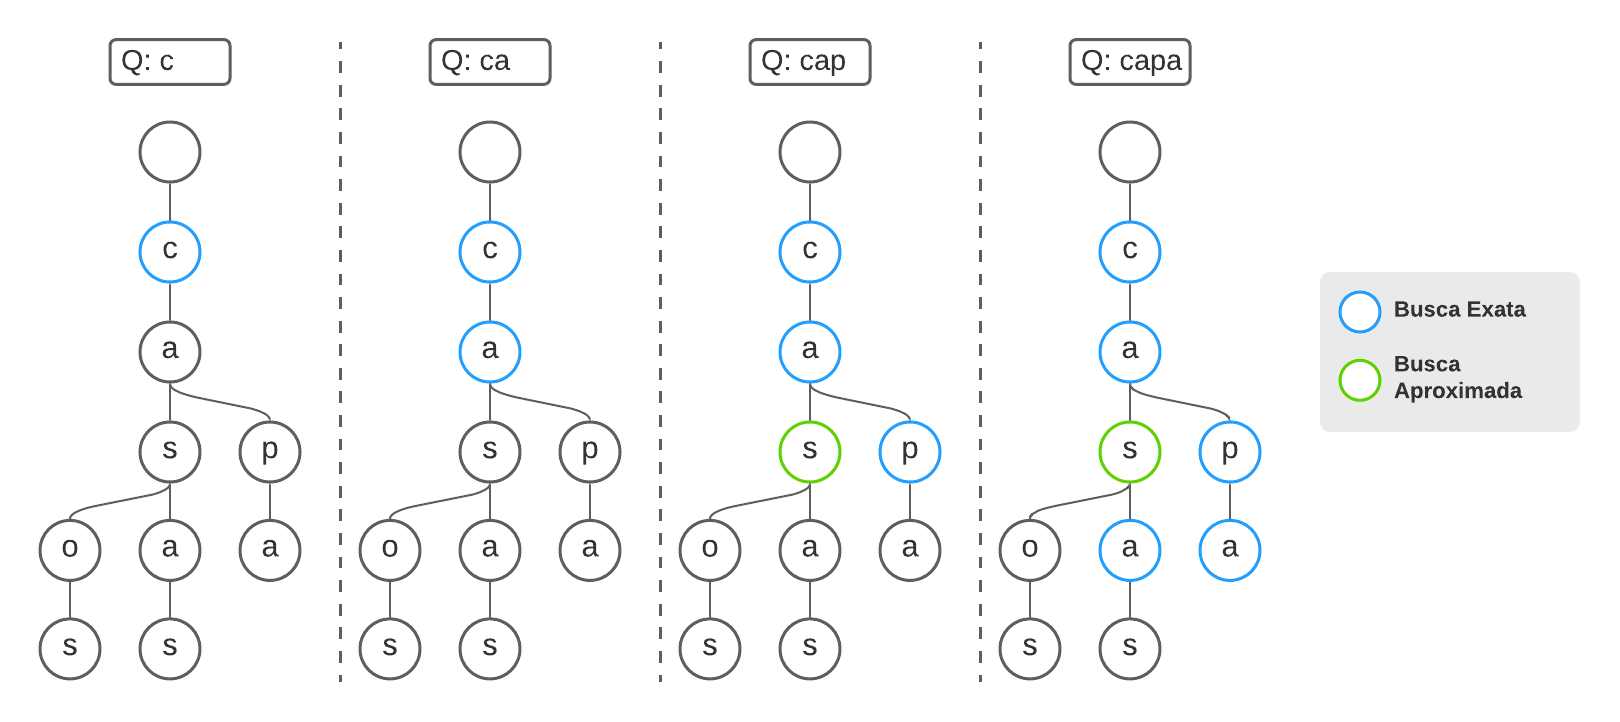
\includegraphics[width=1\textwidth]{figures/trie_exact_and_approximate_search.png}
    \caption{Árvore \textit{Trie} com exemplo de busca exata e aproximada pelo prefixo de consulta ``capa''. Os nós com o contorno azul representam o caminho realizado pela busca exata, e os nós com contorno verde o caminho realizado pela busca aproximada. O caminho da busca aproximada pode conter nós do caminho da busca exata. Esse exemplo considera $\tau = 1$. }
    \label{fig:exact_and_approximate_search_trie}
\end{figure}

Além da busca exata por palavras na \textit{Trie}, também é possível realizar busca aproximada, ou seja, tolerante a erros de digitação. A Figura~\ref{fig:exact_and_approximate_search_trie} mostra um exemplo de busca exata e busca aproximada pelo prefixo de consulta ``capa'' em uma \textit{Trie}. A busca exata consiste em visitar apenas os nós da \textit{Trie} cujos prefixos estão contidos exatamente no prefixo de consulta. Já na busca aproximada, é necessário visitar nós ``vizinhos'' para encontrar prefixos similares que se encontram dentro de um limiar $\tau$. Essa necessidade aumenta bastante a complexidade de processamento das consultas. 

Os prefixos da \textit{Trie} que se encontram dentro do limiar $\tau$ de tolerância de erros são chamados de ``nós ativos'', e a busca aproximada é realizada de forma incremental a partir dos nós ativos do prefixo de consulta anterior. A Figura~\ref{fig:exact_and_approximate_search_trie} contém apenas uma exemplificação de apenas alguns nós que podem ser ativos durante o processamento incremental do prefixo de consulta ``capa'', mas não todos. A forma completa de processamento dos nós ativos será mais detalhada a seguir.

\subsection{Nós Ativos}
\label{sec:active_nodes}

\begin{figure}[ht]
    \centering
    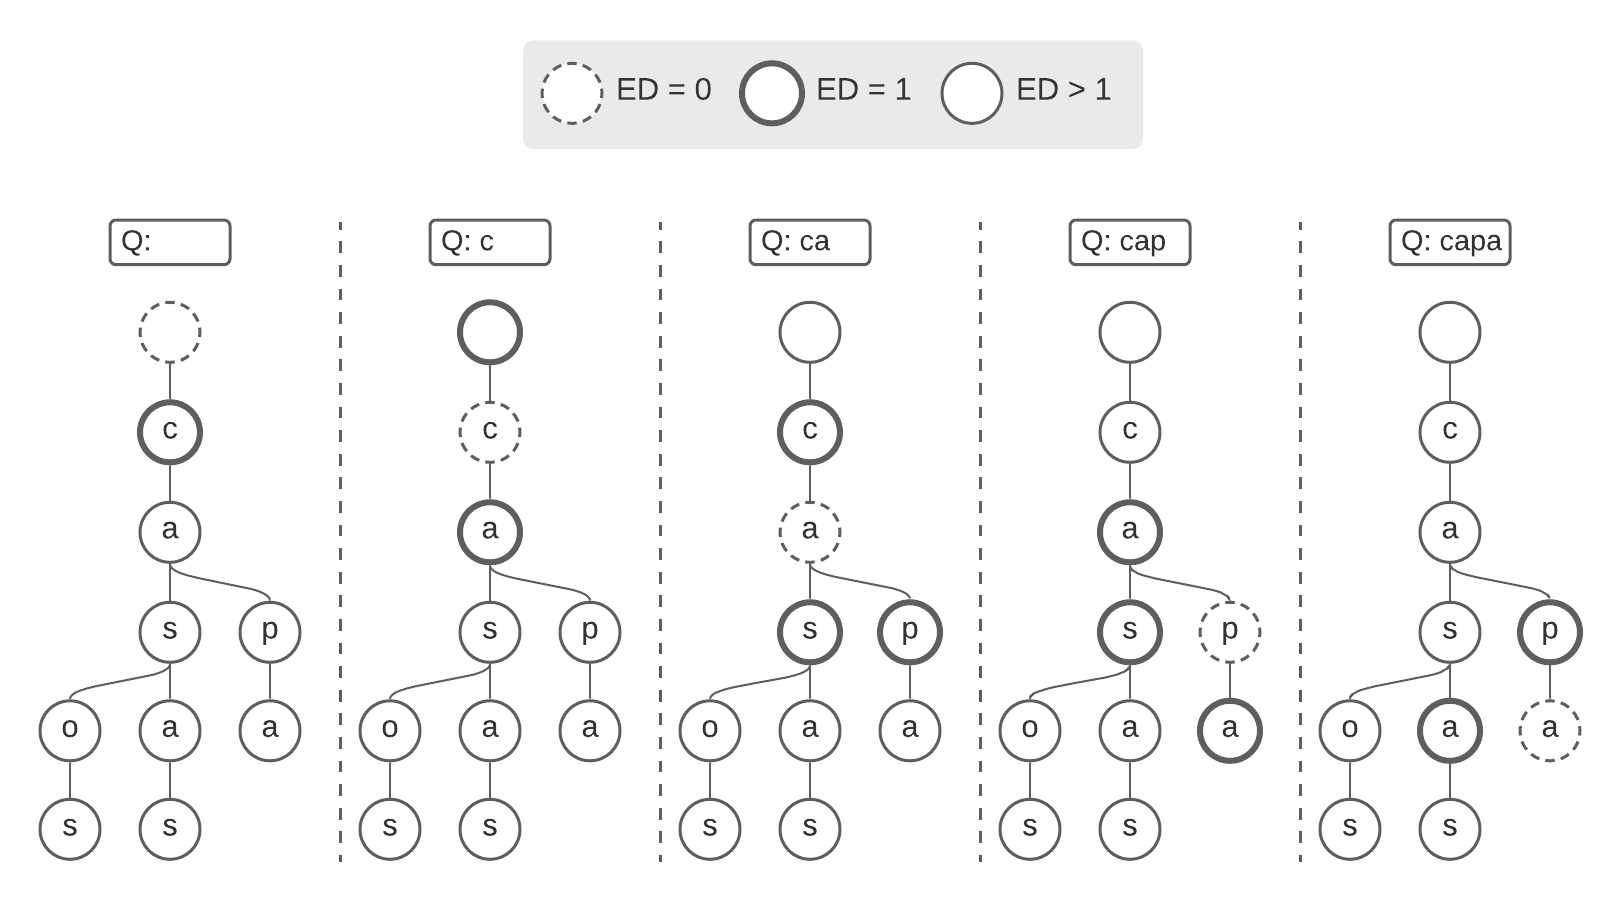
\includegraphics[width=1\textwidth]{figures/trie_active_nodes_example.png}
    \caption{Exemplo de ativação de nós da \textit{Trie} durante o processamento do prefixo de consulta $p = ``capa"$, considerando $\tau = 1$. }
    \label{fig:active_nodes_example}
\end{figure}

Um nó é considerado ativo quando a distância de edição entre seu prefixo e o prefixo consultado é menor ou igual ao limite $\tau$ considerado. O conjunto de nós ativos para um prefixo de consulta $p$ é definido como $V_{p} = \{p_{d} | p_{d} \in P(D) \land ed(p_{d}, p) \leq \tau \}$, onde $P(D)$ é o conjunto de prefixos da base de dados $D$, $p_{d}$ é um prefixo pertencente a $P(D)$ e $p$ é o prefixo de consulta. 

A Figura~\ref{fig:active_nodes_example} demonstra um exemplo de ativação de nós do índice \textit{Trie} à medida que o processamento do prefixo de consulta ``capa'' vai ocorrendo. O limiar de erros tolerados é $\tau = 1$. No início do processamento, considera-se o termo consultado como sendo uma cadeia de caracteres vazia, cujo valor é representado por $\epsilon$. A partir disso, é necessário ativar todos os nós (prefixos) da \textit{Trie} cujos prefixos possam ser transformados no prefixo de consulta, o qual é $\epsilon$ inicialmente. Portanto, os prefixos $\epsilon$ (representado pelo nó raiz da \textit{Trie}) e ``c'' são considerados nós ativos, pois $ed(\epsilon, \epsilon) = 0$ (círculo tracejado) e $ed(``l", \epsilon) = 1$ (círculo de borda grossa). Após isso, o prefixo consultado passa a ser primeira letra de ``capa'', ``c''. Então, é necessário analisar os nós já ativos (e seus respectivos filhos) do prefixo consultado anteriormente para computar os novos nós ativos para ``c''. A análise de cada nó ativo termina quando se encontra um prefixo fora do limiar $\tau$. Os novos nós ativos computados são $\epsilon$, ``c'' e ``ca'', porque $ed(\epsilon, ``c"") = 1$, $ed(``c", ``c"") = 0$ e $ed(``ca", ``c"") = 1$. Todos os outros prefixos além desse possuem distância de edição maior que o limite $\tau = 1$, portanto não são considerados nós ativos. Quando o prefixo de consulta passa a ser ``ca'', o nó raiz já não é mais um nó ativo, pois $ed(\epsilon, ``ca") = 2$, o nó ``c'' continua como nó ativo porém agora com uma distância igual a $1$ em relação a ``ca'', e dois novos nós são ativos, sendo eles  ``cas'' e ``cap'', ambos com distância igual a $1$ também. Esse algoritmo é repetido até chegar no final do prefixo de consulta ``capa'', cujos nós ativos são ``casa'' e ``capa''. O objetivo de computar nós ativos é o de utilizá-los para identificar itens similares ao prefixo consultado.

\section{ICAN}

O algoritmo proposto por \cite{ji2009efficient} denomina-se ``Computando Nós Ativos Incrementalmente'' (\textit{Incrementally Computing Active Nodes } -- ICAN). Considerando uma consulta de prefixo $p$ com apenas uma palavra-chave, para processar os nós ativos de forma eficiente é necessário computar e armazenar um conjunto de tuplas $\Phi_{p} = \{ \langle n, \xi_{n} \rangle \}$ tal que (1) cada $n$ é um nó ativo em relação à $p$ com $\xi_{n} = ed(n, p) \leq \tau)$ e (2) quaisquer nós ativos de $p$ estão presentes em $\Phi_{p}$, que é o \textit{conjunto de nós ativos de p} \citep{ji2009efficient}. Quando o usuário digita mais um caractere $p + 1$ após ter digitado $p$, o conjunto $\Phi_{p}$ de nós ativos de $p$ pode ser usado para computar o conjunto $\Phi_{p + 1}$ de nós ativos da nova consulta.

\subsection{Descrição do Algoritmo}

\begin{figure}[ht]
    \centering
    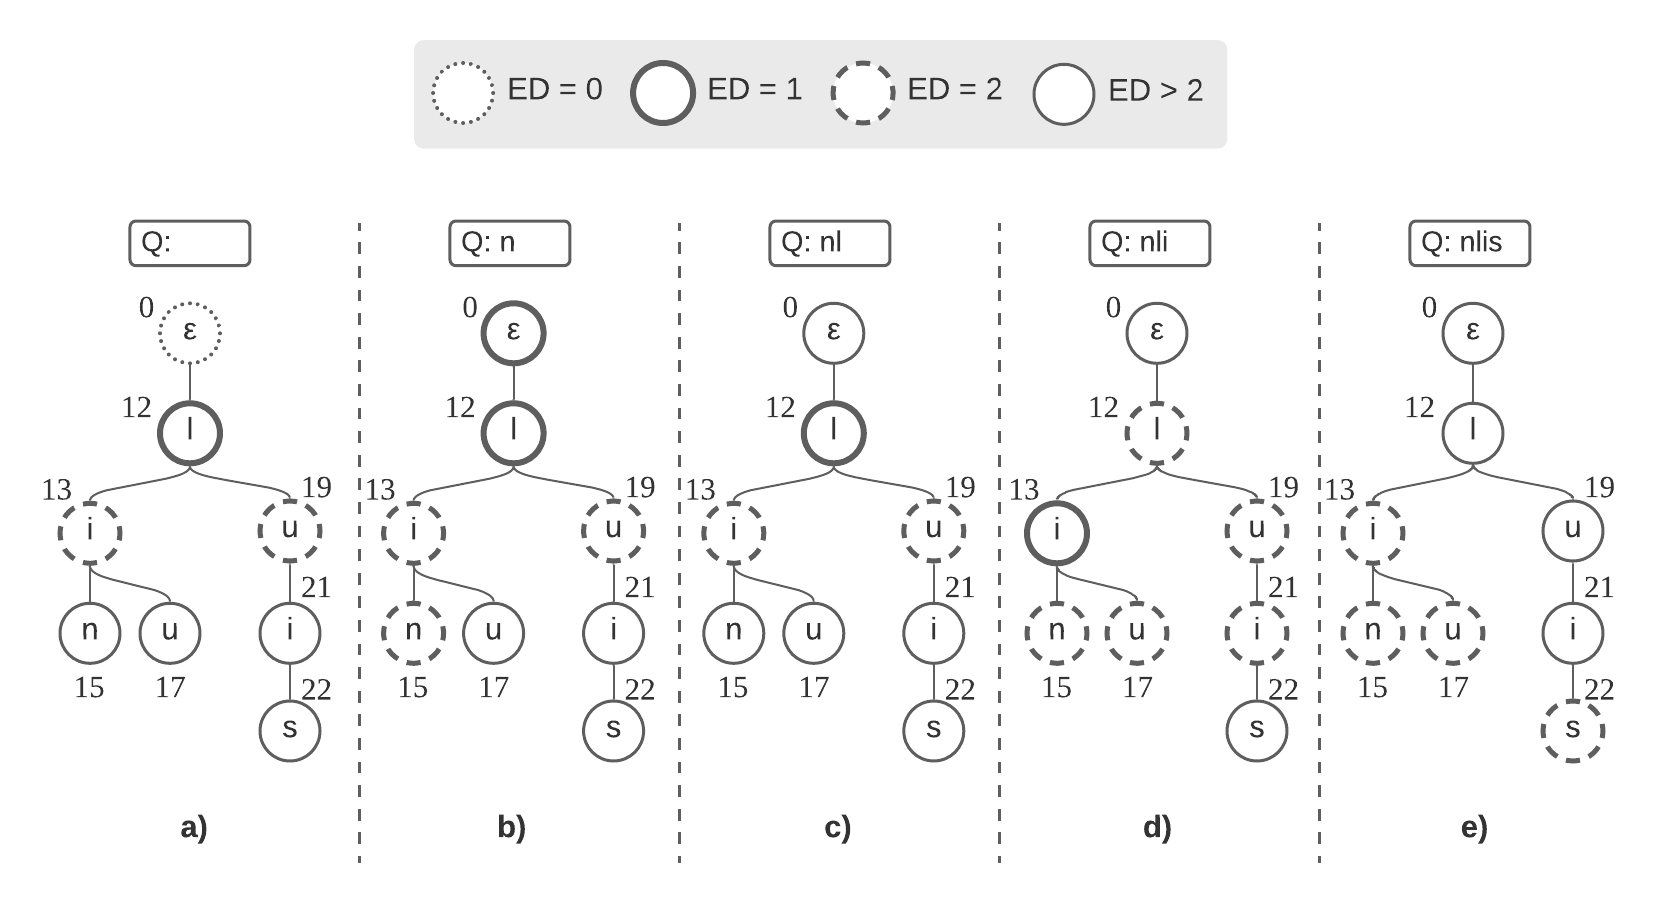
\includegraphics[width=1\textwidth]{figures/ican_example.png}
    \caption{Busca aproximada pelo prefixo de consulta ``nlis'' em uma \textit{Trie}, considerando o limiar de distância de edição $\tau = 2$. \textbf{(a)} Inicialização; \textbf{(b)} consulta por ``n''; \textbf{(c)} consulta por ``nl''; \textbf{(d)} consulta por ``nli''; \textbf{(e)} consulta por ``nlis'' }
    \label{fig:ican_example}
\end{figure}

Antes do usuário digitar qualquer caractere, o prefixo de consulta é considerado uma cadeia vazia $\epsilon$, o qual possui um conjunto de nós ativos $\Phi_{\epsilon}$ correspondente, que é inicializado como $\Phi_{\epsilon} = \{\langle n, \xi_{n} \rangle \mid \xi_{n} = |n| \leq \tau\}$. Esse conjunto inclui todos os nós $n$ da \textit{Trie} cujos prefixos correspondentes possuem um tamanho $|n|$ que é menor ou igual ao limiar $\tau$. No exemplo da Figura~\ref{fig:ican_example}, o primeiro passo é inicializar o conjunto $\Phi_{\epsilon} = \{ \langle n_{0}, 0\rangle, \langle n_{12}, 1\rangle,  \langle n_{13}, 2\rangle,  \langle n_{19}, 2\rangle \}$

\begin{figure}[ht]
    \centering
    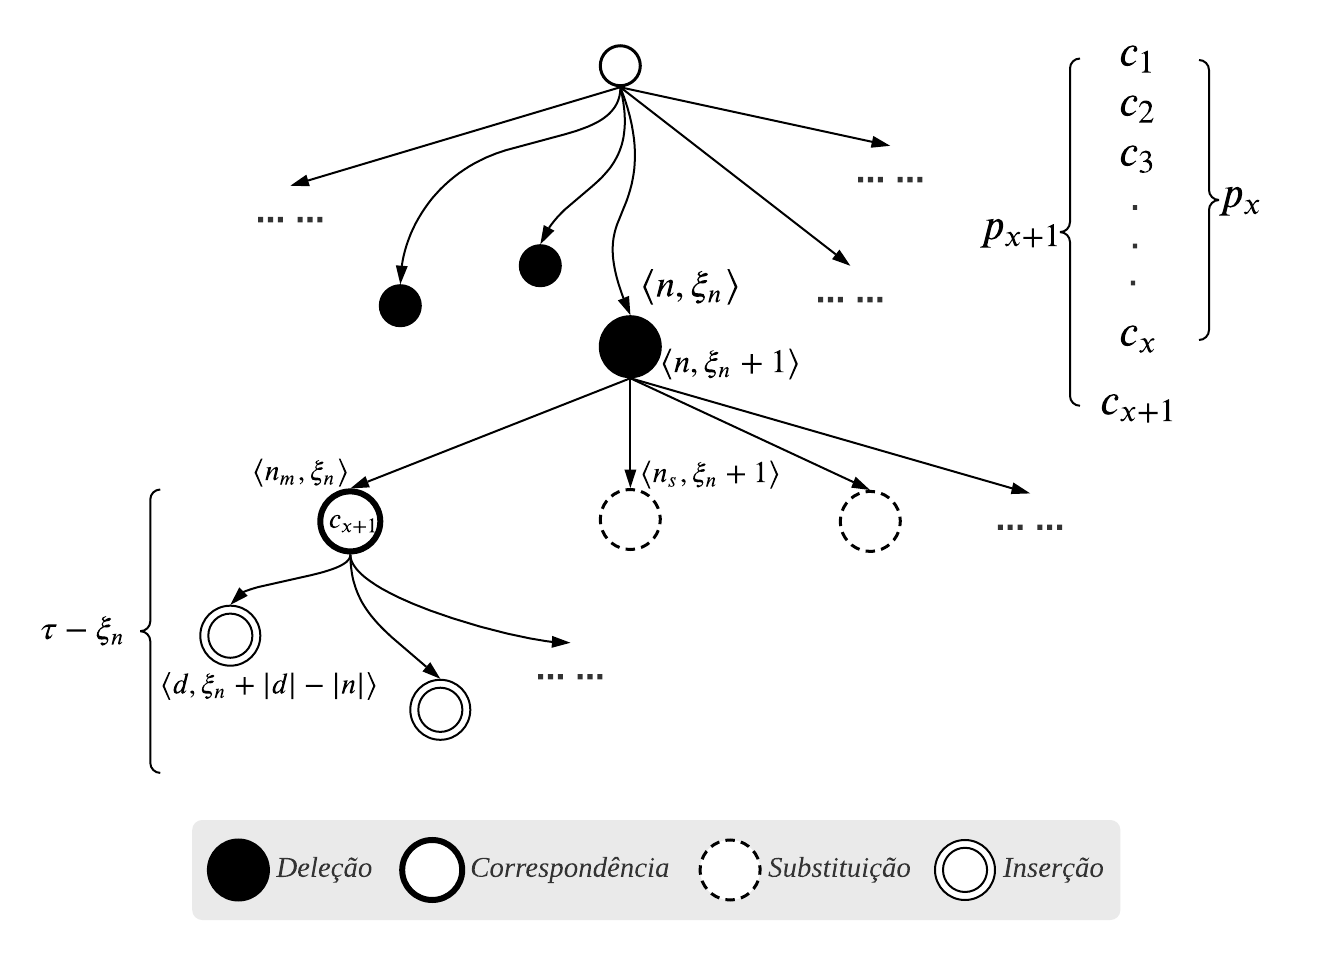
\includegraphics[width=1\textwidth]{figures/incrementally_computing_active_node_set.png}
    \caption{Computação incremental do conjunto de nós ativos $\Phi_{p_{x+1}}$ a partir do conjunto $\Phi{p_{x}}.$ O nó ativo de $\Phi{p_{x+1}}$ considerado é $\langle n, \xi_{n} \rangle$.}
    \label{fig:incrementally_computing_active_node_set}
\end{figure}

Suponhamos que após o usuário digitar o prefixo de consulta $p_{x} = c_{1}c_{2}...c_{x}$, o conjunto de nós ativos $\Phi_{p_{x}}$ para $p_{x}$ é computado. Quando o usuário digitar um novo caractere $c_{x+1}$ e formar um novo prefixo de consulta $p_{x+1}$, o algoritmo computa o conjunto $\Phi_{p_{x+1}}$ para $p_{x+1}$ a partir de $\Phi{p_{x}}$ da seguinte maneira: inicialmente, inicializa-se $\Phi{p_{x+1}}$ como um conjunto vazio; então, para cada tupla $\langle n, \xi_{n} \rangle$ em $\Phi_{p_{x}}$, apenas os descendentes de $n$ são examinados como candidatos de nós ativos para $p_{x+1}$, como é ilustrado na Figura~\ref{fig:incrementally_computing_active_node_set}. Nesse processo, é preciso atentar para os seguintes casos:

\textit{Considerando o nó $n$}: Seja $n$ um nó ativo de $p_{x}$. É possível transformar $n$ para $p_{x+1}$ com $\xi_{n} + 1$ operações de edição ao realizar primeiro uma transformação de $n$ para $p_{x}$ (com $\xi_{n}$ operações) e então deletar o último caractere $c_{x+1}$. Se $\xi_{n} \leq \tau$, então adicionamos a tupla $\langle n, \xi_{n} + 1 \rangle$ em $\Phi_{x + 1}$. Considerando a tupla $\langle n_{0}, 0 \rangle \in \Phi_{\epsilon}$ no exemplo da Figura~\ref{fig:ican_example}, quando o usuário digita o primeiro caractere ``n'' adiciona-se $\langle n_{0}, 1 \rangle$ em $\Phi_{n}$, pois é possível realizar uma operação de deleção na letra ``n'' com distância de edição igual a $1$. É importante ressaltar que devido à igualdade $\Phi_{p_{x}} = \Phi_{c_{1}c_{2}..c_{x}}$, o símbolo $\Phi_{n}$ nesse contexto refere-se ao \textit{conjunto de nós ativos para o prefixo de consulta ``n''}, e não possui relação com a variável $n$ utilizada para representar nós da \textit{Trie} anteriormente.

\textit{Considerando os filhos do nó $n$}: Para cada filho $n_{c}$ de um nó $n$, há dois possíveis casos:

\textit{Caso 1}: O nó filho $n_{c}$ tem um caractere diferente de $c_{x+1}$. A Figura~\ref{fig:incrementally_computing_active_node_set} mostra um nó $n_{s}$, onde ``s'' refere-se à operação de \textit{substituição}. É possível transformar $n_{s}$ em $p_{x+1}$ com $\xi_{n} + 1$ operações ao transformar primeiro $n$ em $p_{x}$ (com $\xi_{n}$ operações) e então substituir o caractere de $n_{s}$ por $c_{x+1}$. Se $\xi_{n} + 1 \leq \tau$ então adiciona-se $\langle n_{s}, \xi_{n} + 1 \rangle$ em $\Phi_{p_{x+1}}$. Esse caso corresponde a substituir o caractere de $n_{s}$ por $c_{x+1}$. No exemplo da Figura~\ref{fig:ican_example}, consideremos o caso em que o usuário digita o primeiro caractere ``n''. Para $\langle n_{0}, 0 \rangle \in \Phi_{\epsilon}$, o nó $12$ é filho do nó $0$ e possui a letra ``l''. Uma vez que é possível aplicar uma operação de substituição de ``l'' por ``n'' com $1$ operação  edição, adiciona-se $\langle n_{12}, 1 \rangle$ em $\Phi_{n}$. 

\textit{Caso 2}: O nó filho $n_{c}$ possui um caractere que corresponde ao caractere $c_{x+1}$ (o caractere de $n_{c}$ é igual a $c_{x+1}$). A Figura~\ref{fig:incrementally_computing_active_node_set} mostra o nó $n_{m}$, onde ``m'' refere-se à operação de \textit{correspondência}. É possível transformar $n_{m}$ para $p_{x+1}$ com $\xi_{n}$ operações ao transformar primeiro $n$ em $p_{x}$ (com $\xi_{n}$ operações) e então igualando o caractere de $n_{m}$ com $c_{x+1}$. Adiciona-se $\langle n_{m}, \xi_{n} \rangle$ em $\Phi_{p_{x+1}}$. Adicionalmente, se $\xi_{n} < \tau$ então as seguintes operações também são necessárias: para cada descendente $d$ de $n_{m}$ que dista no máximo $\tau - \xi_{n}$ letras de $n_{m}$, é preciso adicionar $\langle d, \xi_{d} \rangle$ em $\Phi_{p_{x+1}}$, sendo $\xi_{d} = \xi_{n} + |d| - |n_{m}|$. No exemplo da Figura~\ref{fig:ican_example}, suponhamos que o usuário digite o primeiro caractere ``l''. Para $\langle n_{0}, 0 \rangle \in \Phi_{\epsilon}$, o nó $12$ é filho do nó $0$ e possui a letra ``l''. Uma vez que o caractere do nó $12$ corresponde ao caractere ``l'', $\langle n_{12}, 0 \rangle$ é adicionado em $\Phi_{l}$. Além disso, o nó $13$ é filho do nó $13$. Uma vez que é possível adicionar o caractere de $n_{13}$ (``i'') após o nó $12$ com $1$ operação de edição, adiciona-se $\langle n_{13}, 1 \rangle$ em $\Phi_{l}$.

Para manter apenas as distâncias de edição mínimas no conjunto de nós ativos, durante a computação de $\Phi_{p_{x+1}}$, toda vez que se deseja adicionar uma tupla $\langle v, \xi_{1} \rangle$ ao conjunto é possível que o mesmo já contenha a tupla $\langle v, \xi_{2} \rangle$ para o mesmo nó $v$ no conjunto. Então, se $\xi_{1} \geq \xi_{2}$ a nova tupla não é adicionada. Se $\xi_{1} < \xi_{2}$, então a nova tupla substitui a original no conjunto. Ou seja, para um mesmo nó $v$ da \textit{Trie} no novo conjunto mantém-se apenas a sua menor distância de transformação para o prefixo de consulta $p_{x+1}$.

\section{ICPAN}

De acordo com o que foi dito na seção~\ref{sec:active_nodes}, o principal propósito de computar os nós ativos é usá-los para identificar itens similares ao prefixo consultado. Considerando o algoritmo ICAN, o conjunto de nós ativos final para o prefixo de consulta pode acabar sendo muito grande, o que aumenta o tempo de processamento. Diante desse problema \cite{li2011efficient} propuseram uma melhoria no algoritmo que consiste em podar nós ativos desnecessários, mas ainda mantendo a possibilidade de computar as respostas à consulta. As principais vantagens desse método são a redução do espaço de memória necessário para armazenar o conjunto de nós ativos, e também a redução do tempo de processamento da consulta, pois não é necessário examinar todos os nós ativos. 
Segue um exemplo de poda que reflete a intuição por trás desse método. Ainda considerando o exemplo da Figura~\ref{fig:incrementally_computing_active_node_set}, seja ``nl'' prefixo consultado com um limiar $\tau = 2$, onde $\Phi_{nl} = \{ \langle n_{12}, 1\rangle, \langle n_{0}, 2\rangle,  \langle n_{13}, 2\rangle,  \langle n_{19}, 2\rangle \}$. No entanto, apesar de $n_{13}$ (``li'') e $n_{19}$ (``lu'') serem nós ativos, não é necessário mantê-los, pois é possível utilizar o nó ativo $n_{12}$ (``l'') para computar as palavras ``li'' e ``lu''. Ou seja, é necessário manter apenas o nó ativo ``l'' para computar o mesmo conjunto de itens similares ao prefixo ``nl'' consultado.

\subsection{Nós Pivô Ativos}
\label{sec:pivotal_active_nodes}

Seja $n$ um nó ativo de $p$. Se para qualquer transformação de $n$ para $p$ com $ed(n,p)$ operações a operação no último caractere de $n$ não for uma correspondência (caracteres iguais), e for possível deletar o último caractere de $n$, o nó $n$ não é mantido, e sim o seu nó pai. Assim, surge o conceito de \textit{nó pivô ativo} \citep{li2011efficient}.

Considerando novamente o prefixo ``nl'' no exemplo da Figura~\ref{fig:incrementally_computing_active_node_set}, sabe-se que ``l'' é um nó ativo, e que ``li'' e ``lu'' são nós ativos cuja distância de edição entre ``nl'' é igual a $2$, e seus últimos caracteres não correspondem aos caracteres do prefixo ``nl''. É possível derivar esses dois nós ativos a partir do nó ``l'' ao inserir os caracteres ``i'' e ``u'', respectivamente. Além disso, também é possível computar as palavras similares ``li'' e ``lu'' ao visitar os nós folhas que são descendentes de ``l''. Portanto, não é necessário manter esses dois nós ativos. Nesse exemplo, o nó ``l'' é chamado \textit{nó pivô ativo}, pois serve como ``pivô'' para computar outras palavras similares à consulta sem a necessidade de ativar mais nós. Para um prefixo de consulta $p$, um nó $n$ é um nó pivô ativo de $p$ em relação ao limiar de distância de edição $tau$, se e somente se $n$ for um nó ativo de $p$ e se existir uma transformação de $p$ em $n$ com $ed(n,p)$ operações de edição, e a operação no último caractere de $n$ for a de correspondência. Ou seja, a operação no último caractere de $n$ não é nem uma deleção $ed(n,p) \neq ed(n', p) + 1$ e nem uma substituição $ed(n,p) \neq ed(n', p') + 1$, onde $n'$ e $p'$ são respectivamente os prefixos de $n$ e $p$ que não contêm o último caractere. 

Para computar de forma eficiente os nós pivô ativos, \cite{li2011efficient} desenvolveram o algortimo ``Computando Nós Pivô Ativos Incrementalmente'' (\textit{Incrementally Computing Pivotal Active Nodes } -- ICPAN). Sendo $p_{x}$ um prefixo de consulta, o objetivo é computar e armazenar um conjunto de 4-uplas $\Psi_{p_{x}} = \{ \langle n, \xi_{n}^{p_{x}}, p_{i}, \xi_{n}^{p_{i}} \rangle \}$. Em cada 4-upla do conjunto, $n$ é um nó pivô ativo de $p_{x}$, e \textit{$p_{i}$ é um prefixo de $p_{x}$ cujos últimos caracteres são iguais aos últimos caracteres de $n$}. Se esse prefixo não existir, então $p_{i} = \epsilon$. Se houver mais de uma possibilidade para $p_{i}$, então seleciona-se aquele com o menor número de caracteres. O quarto elemento da tupla, $\xi_{n}^{p_{i}} \leq \tau$ é a distância de dição entre o nó $n$ e o prefixo $p_{i}$ com operações de correspondência entre os últimos caracteres de $n$ e $p_{i}$. Já o segundo elemento da tupla, $\xi_{n}^{p_{x}} \leq \tau$ é a distância de edição entre nó $n$ e o prefixo de consulta $p_{x}$, obtida transformando primeiro $n$ em $p_{i}$, e então inserindo os caracteres restantes da diferença entre $p_{x}$ e $p_{i}$. A partir disso, deriva-se a igualdade $\xi_{n}^{p_{x}}=\xi_{n}^{p_{i}} + |p_{x}|-|p_{i}|$.

\subsection{Descrição do Algoritmo}
\label{sec:icpan_algorithm_description}

Antes do usuário digitar qualquer caractere, o prefixo de consulta é considerado uma cadeia vazia $\epsilon$, e então seu conjunto de nós pivô ativos correspondente é inicializado como $\Psi_{\epsilon} = \{ \langle r, 0, \epsilon, 0 \rangle \}$, onde $r$ é o nó raiz, já que a raiz é o único nó pivô ativo para $\epsilon$ de acordo com as definições estabelecidas anteriormente. Considerando ainda o mesmo exemplo da Figura~\ref{fig:incrementally_computing_active_node_set}, no qual o usuário digita o prefixo de consulta ``nlis'' caractere a caractere, e o limiar de distância de edição é $\tau = 2$, o primeiro passo é inicializar o conjunto como $\Psi_{\epsilon} = \{ \langle n_{0}, 0, \epsilon, 0 \rangle \}$, sendo $n_{0}$ o nó raiz. 

\begin{figure}[ht]
    \centering
    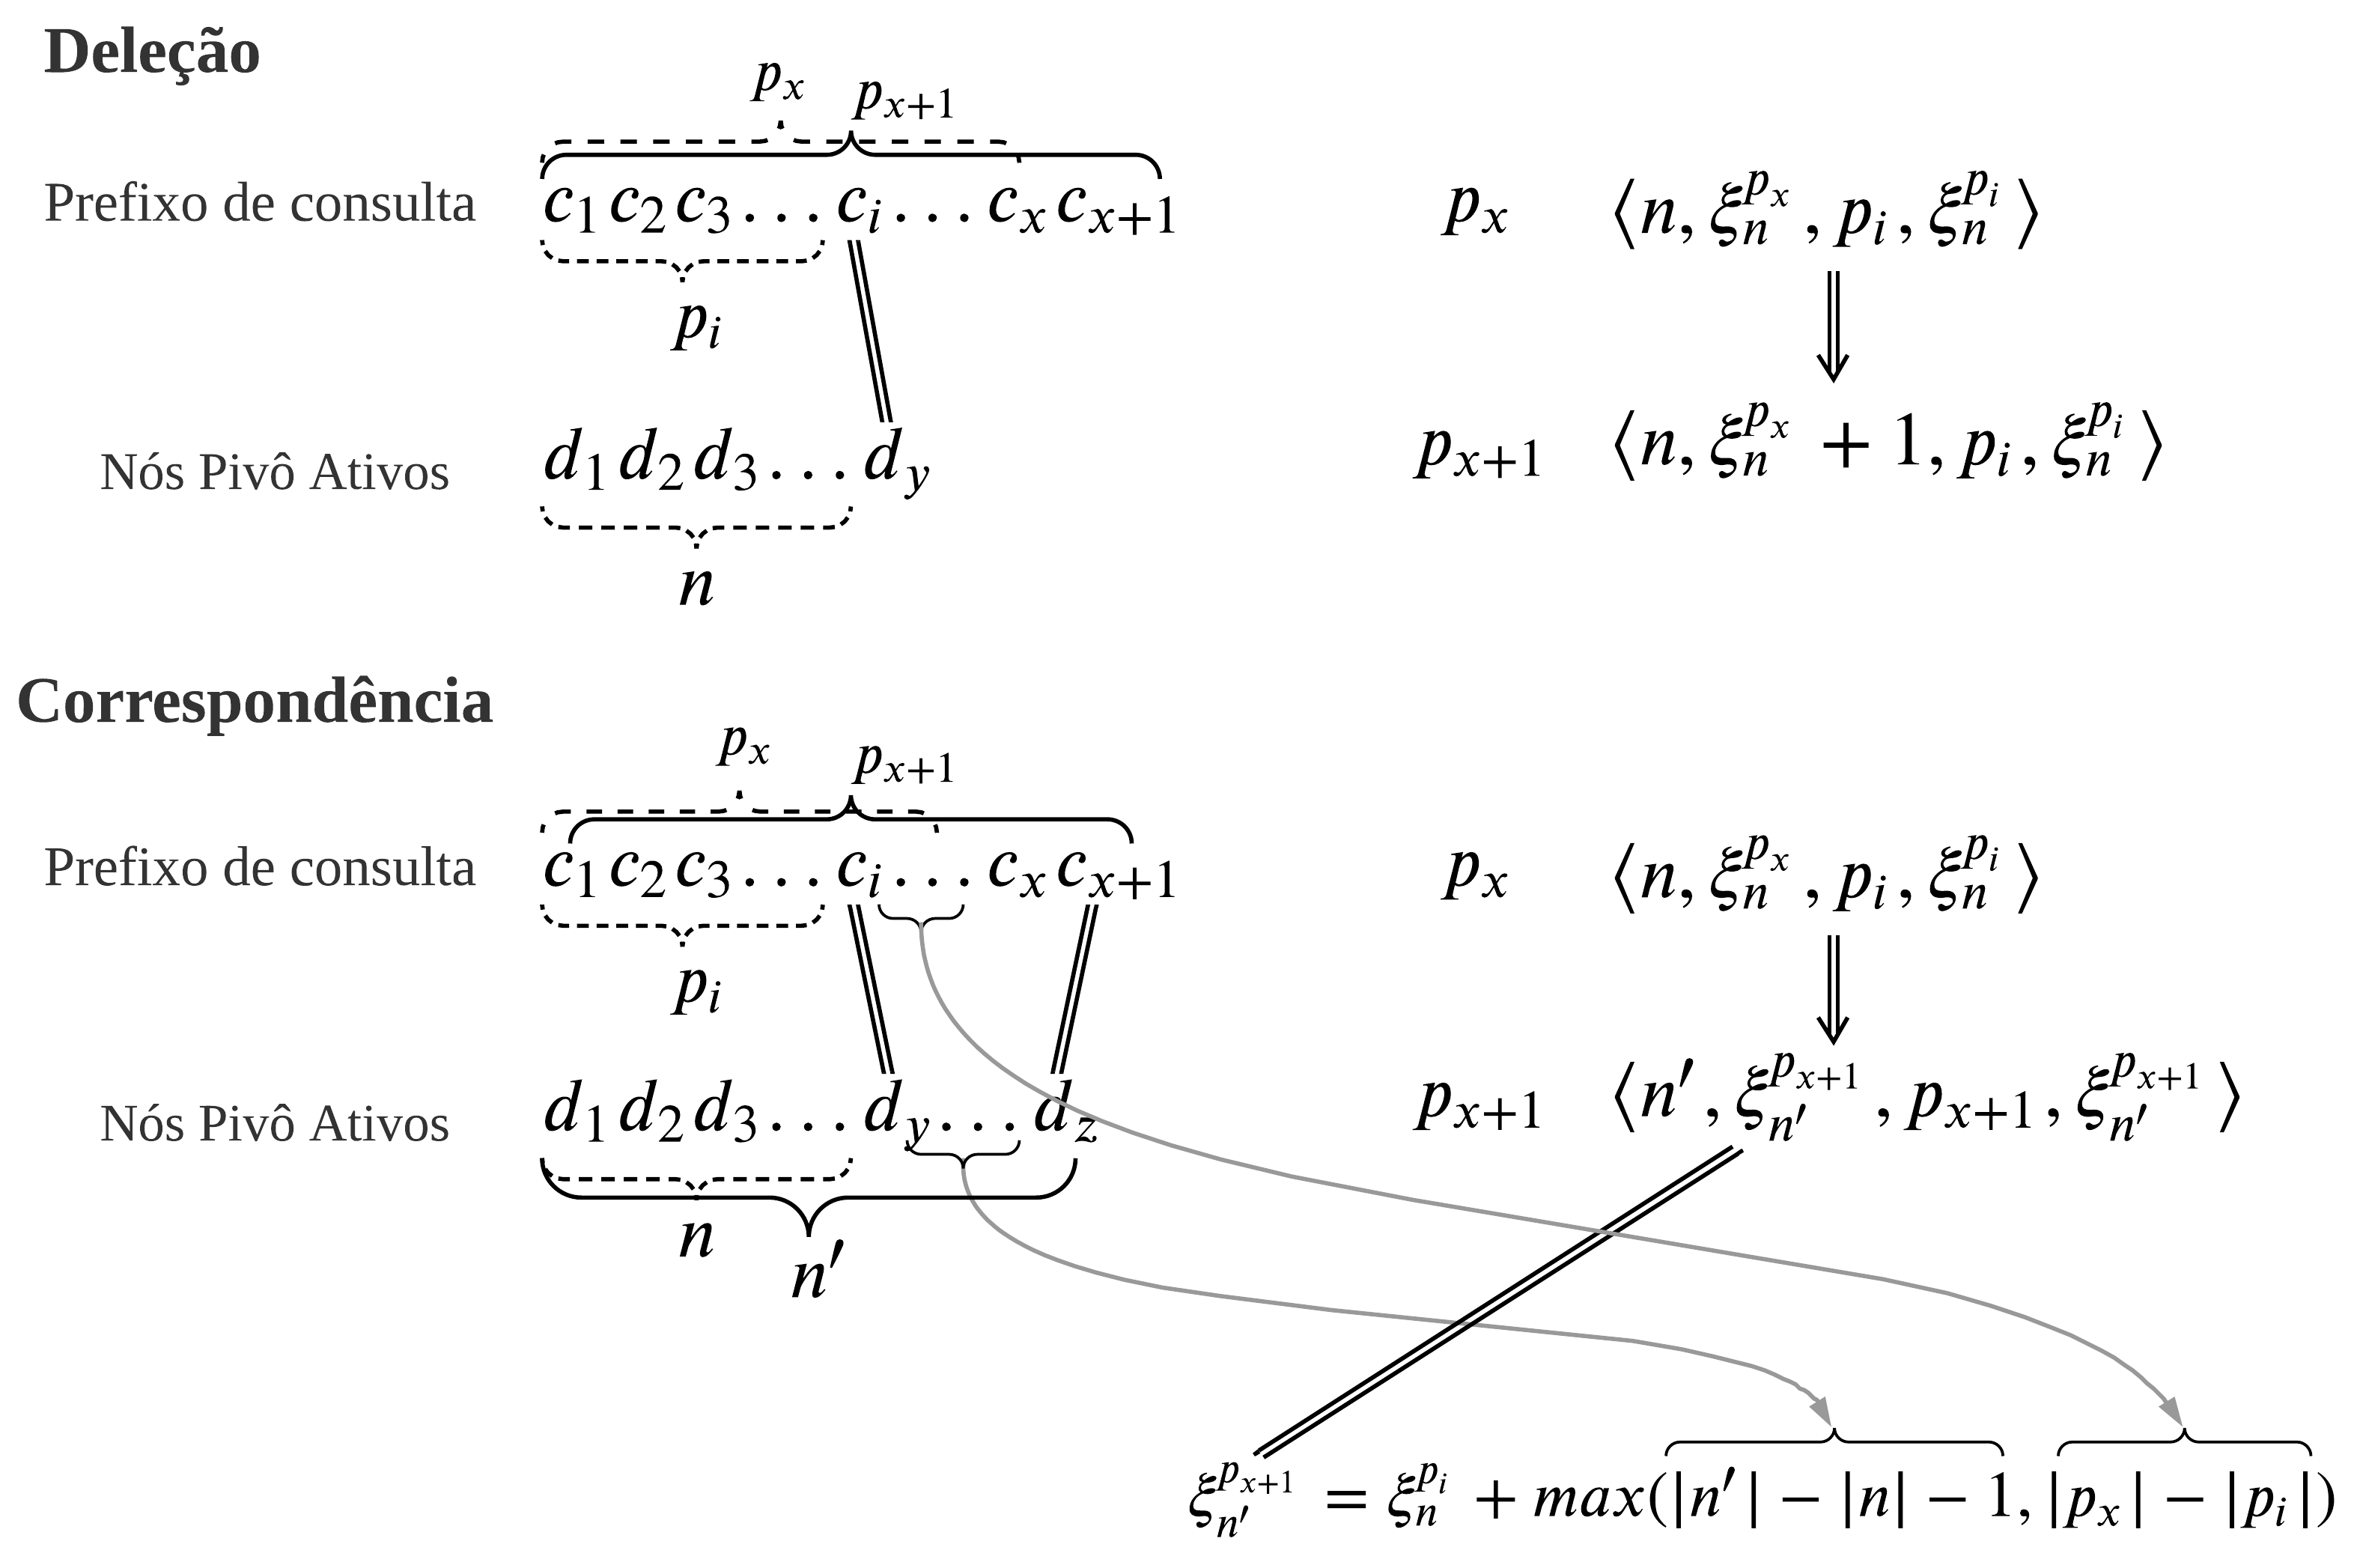
\includegraphics[width=1\textwidth]{figures/incrementally_computing_pivotal_nodes.png}
    \caption{Computação incremental de nós pivô ativos, sendo $c_{i} = d_{y}$ e $c_{x+1} = d_{z}$.}
    \label{fig:incrementally_computing_pivotal_nodes}
\end{figure}

Suponhamos que após o usuário digitar o prefixo de consulta $p_{x} = c_{1}c_{2}...c_{x}$, o conjunto de nós ativos $\Psi_{p_{x}}$ para $p_{x}$ é computado. Quando o usuário digitar um novo caractere $c_{x+1}$ e formar um novo prefixo de consulta $p_{x+1}$, o algoritmo computa o conjunto $\Psi_{p_{x+1}}$ para $p_{x+1}$ a partir de $\Psi{p_{x}}$ da seguinte maneira: inicialmente, inicializa-se $\Psi{p_{x+1}}$ como um conjunto vazio; então, para cada 4-upla $ \langle n, \xi_{n}^{p_{x}}, p_{i}, \xi_{n}^{p_{i}} \rangle$, apenas os descendentes de $n$ são examinados como candidatos de nós pivô ativos para $p_{x+1}$, como é ilustrado na Figura~\ref{fig:incrementally_computing_pivotal_nodes}. Nesse processo, é preciso atentar para os seguintes casos (todos os exemplos a seguir também consideram a árvore \textit{Trie} da Figura~\ref{fig:ican_example}):

\textit{Considerando o nó n}: Seja $n$ um nó pivô ativo de $p_{x}$. É possível transformar $n$ em $p_{x+1}$ com $\xi_{n}^{p_{x}} + 1$ operações de edição ao primeiro transformar $n$ em $p_{x}$ (com $\xi_{n}^{p_{x}}$ operações) e então deletar o último caractere $c_{x+1}$. Se $\xi_{n}^{p_{x}} + 1 \leq \tau$, então adiciona-se $\langle n, \xi_{n}^{p_{x}} + 1, p_{i}, \xi_{n}^{p_{i}} \rangle$ ao conjunto $\Psi_{p_{x+1}}$. Se o usuário digitar ``n'' por exemplo, uma vez que é possível realizar uma operação de deleção do caractere ``n'' com $1$ operação de edição, a partir da 4-upla $\langle n_{0}, 0, \epsilon, 0 \rangle \in \Psi_{\epsilon}$ é possível adicionar $\langle n_{0}, 1, \epsilon, 0 \rangle$ em $\Psi_{n}$.

\textit{Considerando os descendentes do nó n}: Consideremos os descendentes de $n$ \textit{que possuem o caractere $c_{x+1}$} e que não distem de $n$ mais do que $\tau - \xi_{n}^{p_{i}} + 1$ passos. Para esse descendente $n'$ nessa condição, é possível transformar $n'$ em $p_{x+1}$ com os seguintes passos: (1) transformar $n$ em $p_{i}$; (2) transformar os caracteres após $n$ e antes de $n'$ nos caracteres $c_{i+1}...c_{x}$; e (3) verificando a operação de correspondência do caractere $n'$ com $c_{x+1}$. Isso implica que é possível transformar $n'$ em $p_{x+1}$ com $\xi_{n'}^{p_{x+1}} = \xi_{n}^{p_{i}} + max(|n'| - |n| - 1, |p_{x}| - |p_{i}|)$ operações. Se $\xi_{n'}^{p_{x+1}} \leq \tau$, então adiciona-se $\langle n', \xi_{n'}^{p_{x+1}}, p_{x+1}, \xi_{n'}^{p_{x+1}} \rangle$ em $\Psi_{p_{x+1}}$. Por exemplo, se o usuário digitar o primeiro caractere ``n'' e considerando $\langle n_{0}, 0, \epsilon, 0 \rangle \in \Psi_{\epsilon}$, uma vez que o nó $n_{15}$(``lin'') corresponde a ``n'', então adiciona-se $\langle n_{15}, 2, ``lin", 2 \rangle$ em $\Psi_{n}$.

Semelhantemente ao ICAN, também é necessário manter a distância de edição mínima no conjunto de 4-uplas. Durante o processamento do novo conjunto $\Psi_{p_{x+1}}$, para um mesmo nó $n$, mantém-se somente a distância de edição entre o nó $n$ e o prefixo de consulta $p_{x+1}$. Toda vez que se deseja adicionar uma 4-upla $\langle n, \xi_{n}^{p_{x + 1}}, p_{i}, \xi_{n}^{p_{i}} \rangle$ ao conjunto é possível que o mesmo já contenha a 4-upla $\langle n, {\xi'}_{n}^{p_{x + 1}}, p_{j}, {\xi'}_{n}^{p_{j}} \rangle$ para o mesmo nó $n$ no conjunto. Se ${\xi'}_{n}^{p_{x+1}} > \xi_{n}^{p_{x+1}}$, então a nova 4-upla \textit{não é adicionada}. Se ${\xi'}_{n}^{p_{x+1}} = \xi_{n}^{p_{x+1}}$ e $|p_{j}| < |p_{i}|$, então a nova 4-upla substitui a 4-upla original (isso garante que apenas o prefixo com o menor número de caracteres seja mantido, como descrito em \ref{sec:pivotal_active_nodes}). Por fim, se ${\xi'}_{n}^{p_{x+1}} < \xi_{n}^{p_{x+1}}$, então a nova 4-upla \textit{substitui a original que já estava no conjunto}.

O ICPAN possui uma situação a mais para tratar em comparação ao ICAN: a remoção de nós ativos que não são pivôs. Para cada 4-upla $\langle n, \xi_{n}^{p_{x + 1}}, p_{i}, \xi_{n}^{p_{i}} \rangle$, \textbf{se $\mathbf{p_{i} \neq p_{x+1}}$}, então é feita uma verificação para cada nó ``ancestral'' $n_{a} \neq n$ de $n$. Se $\langle n_{a}, \xi_{n_{a}}^{p_{x + 1}}, p_{a}, \xi_{n_{a}}^{p_{a}} \rangle \in \Psi_{p_{x+1}}$ \textit{e} $\xi_{n_{a}}^{p_{a}} + max(|p_{x+1}| - |p_{a}|, |n| - |n_{a}|) < \xi_{n}^{p_{x+1}}$, então é preciso remover $\langle n, \xi_{n}^{p_{x + 1}}, p_{i}, \xi_{n}^{p_{i}} \rangle$ do conjunto. É necessário que isso aconteça pois nessas condições há uma transformação do nó $n$ para $p_{x+1}$ com uma distância de edição menor do que $\xi_{n}^{p_{x+1}}$ sem que haja correspondência no último caractere do nó $n$, ou seja, $n$ não é um nó pivô ativo do prefixo de consulta $p_{x+1}$.

Tanto o ICAN quanto o ICPAN produzem no final do processamento um conjunto de nós ativos. Os dois algoritmos consideram que cada nó folha $n_{folha}$ da árvore \textit{Trie} possui uma lista invertida $L$ de ``\textit{IDs}'' dos itens que possuem o prefixo referente ao nó $n_{folha}$. Então, para cada nó ativo do conjunto final obtido, obtem-se todos os nós folhas dentre seus descendentes. \textit{A lista de \textit{IDs} resultante das interseções entre as listas de todos esses nós folhas obtidos é a lista de itens similares ao prefixo consultado, ou seja, a resposta para o problema de CATE}.

\section{Busca em dois níveis}

Uma possível estratégia de busca em dois níveis para o problema de CATE consiste indexar somente parte dos itens da base de dados em uma árvore \textit{Trie}, e combinar um algoritmo de busca aproximada para essa estrutura (primeiro nível) com o algoritmo de busca sequencial apresentado na seção~\ref{sec:sequential_search} (segundo nível). Para isso, o prefixo de consulta também precisa ser divido em duas partes que são processadas por cada nível. Nessa abordagem, uma vez que os itens são indexados apenas parcialmente, o conjunto de nós ativos obtidos no final da execução do algoritmo do primeiro nível recebe uma nova função. Normalmente, tal conjunto é utilizado para computar os itens similares ao prefixo consultado, mas nessa abordagem de dois níveis, passa a ser usado como filtro para a busca sequencial do segundo nível, que é realizada somente nos itens referenciados por esses nós ativos.
 
\section{Busca binária com elementos repetidos na coleção}
\label{sec:binary_search_with_duplicates}

Considerando a abordagem em dois níveis, neste trabalho analisamos a hipótese de que é possível utilizar não somente busca sequencial no segundo nível, mas também busca binária em alguns casos especiais, que são nós ativos com uma determinada característica explicada com mais detalhes na sessão~\ref{sec:metodo}. Nesses casos, é necessário realizar buscas binárias nas listas invertidas dos nós folha descendentes dos nós ativos.

O melhor algoritmo para busca em vetores ordenados é o de busca binária. Esse método requer que a coleção em que se fará a busca esteja ordenada. A busca binária padrão compara o valor buscado com o valor do elemento que se encontra no meio da coleção. Se eles não forem iguais, a metade da coleção na qual o valor buscado não pode ser encontrado é desconsiderada, e a busca continua na metade restante, considerando novamente o valor do elemento do meio. Esse processo se repete até que o valor seja encontrado. Se a busca terminar e a metade restante estiver vazia, a busca não encontrou o valor. A complexidade da busca binária é $O(\log n)$, enquanto a da busca sequencial é $O(n)$.

Porém, em algumas situações em que coleção possui elementos duplicados, pode ser necessário encontrar não um índice de um valor duplicado qualquer, mas o índice da primeira ocorrência do valor (limite inferior) juntamente com o índice da sua última ocorrência na coleção (limite superior). Para isso é necessário realizar primeiro uma busca binária especializada para encontrar o limite inferior, e depois realizar novamente outra busca binária própria para encontrar o limite superior. Após essas duas buscas, será obtido um intervalo $R = [limInferior, limSuperior]$ referente aos índices da coleção nos quais pode encontrar o valor duplicado que foi buscado. Nas buscas binárias por limite inferior e superior utilizadas no algoritmo~\ref{alg:ip2lb} da seção~\ref{sec:IP2LB}, quando o valor buscado não é encontrado consideramos os limites inferior e superior como sendo negativos, ou seja, $R = [-1, -1]$ por exemplo. 

